\documentclass{book}
\usepackage{graphicx}
\usepackage[english]{babel}
\usepackage{amsthm}
\usepackage{amssymb}
\usepackage{amsfonts}
\usepackage{mdframed}
\usepackage{physics}
\usepackage{tikz}
\usepackage[a4paper, margin=1in]{geometry}
\geometry{a4paper, margin=1in}
\usepackage{xcolor}
\usetikzlibrary{arrows.meta}
\usetikzlibrary{angles,quotes}
\graphicspath{ {./images/} }
\usepackage{svg}
\usepackage{subcaption}
\usepackage{bm}
\usepackage{empheq}
\usepackage{cancel}
\usetikzlibrary{decorations.text}
\usepackage[most]{tcolorbox}
\usepackage{tensor}
%3D
\usepackage{mathtools}
\usepackage{booktabs}
\usepackage{array}
\newcolumntype{C}{>{$}c<{$}}
\usepackage{tikz-3dplot}
\usepackage{appendix}
\usepackage{pgfplots}
\usetikzlibrary{shapes.geometric}
\usetikzlibrary{calc,patterns,angles,quotes}
%Tikz Library
\usetikzlibrary{angles, quotes, intersections}
\usepackage[bb=dsserif]{mathalpha}
\usetikzlibrary{decorations.pathmorphing}

\tikzset{snake it/.style={decorate, decoration=snake}}

\usepackage{etoolbox} % ifthen
\usepackage[outline]{contour} % glow around text
\usetikzlibrary{calc} % for adding up coordinates
\usetikzlibrary{decorations.markings,decorations.pathmorphing}
\usetikzlibrary{angles,quotes} % for pic (angle labels)
\usetikzlibrary{arrows.meta} % for arrow size
\usepackage{xfp} % higher precision (16 digits?)

\usepackage{tcolorbox}

\def\innerproduct#1#2{\langle#1,#2\rangle}

%https://osl.ugr.es/CTAN/macros/latex/contrib/tcolorbox/tcolorbox.pdf
\tcbuselibrary{breakable}
\tcbset{%any default parameters
	width=0.7\textwidth,
	halign=justify,
	center,
	breakable,
	colback=white    
}

\newenvironment{aside}
{\begin{mdframed}[style=0,%
		leftline=false,rightline=false,leftmargin=2em,rightmargin=2em,%
		innerleftmargin=0pt,innerrightmargin=0pt,linewidth=0.75pt,%
		skipabove=7pt,skipbelow=7pt]\small}
	{\end{mdframed}}

\renewcommand{\cleardoublepage}{\clearpage}

\title{Complex Variables and Vector Spaces}
\author{Dominik Szablonski}
\newtheorem{law}{Law}
\newtheorem{klaw}{Law}

\newtcbtheorem{Definitions}{Definition}%
{colback=blue!5!white,colframe=blue!75!black,width=\textwidth,fonttitle=\bfseries}{}

\newtcbtheorem{Theorems}{Theorem}%
{colback=red!5!white,colframe=red!75!black,width=\textwidth,fonttitle=\bfseries}{}

\newtcbtheorem{Examples}{Example}%
{colback=yellow!5!white,colframe=yellow!75!black,width=\textwidth,fonttitle=\bfseries}{}


\newtheorem*{theorem}{Theorem}


\setlength\parindent{0pt}
\pgfplotsset{compat=1.18}
\begin{document}
\maketitle

\tableofcontents

\chapter{Vector Spaces}
We wish to generalise the idea of a vector and field. Let us first define a field,
\begin{Definitions}{Fields}{}
	A field $\mathbb{F}$ is a set with 2 binary operations defined on it, addition $(+)$ and multiplication $(\cdot)$. The following axioms hold $\forall a,b,c \in \mathbb{F}$,
	\begin{enumerate}
		\item \textit{Associativity}, \begin{align}
			a + (b + c) = (a + b) + c &&
			a \cdot (b\cdot c) = (a\cdot b) \cdot c
		\end{align}
		\item \textit{Commutativity}, \begin{align}
			a + b = b + a &&
			a\cdot b = b\cdot a
		\end{align}
		\item \textit{Identity}. $\exists 0, 1 \in \mathbb{F}$ such that,
		\begin{align}
			a + 0 = a &&
			a\cdot 1 = a
		\end{align}
		\item \textit{Additive inverse.} $\forall a \in \mathbb{F}, \exists -a \in \mathbb{F}$ such that,
		\begin{equation}
			a + (-a) = 0.
		\end{equation}
		\item \textit{Multiplicative inverse.} $\forall a \in \mathbb{F}, \exists a^{-1} \in \mathbb{F}$ such that,
		\begin{equation}
			a \cdot a^{-1} = 1.
		\end{equation}
	\end{enumerate}
\end{Definitions}
We can then define a vector space,
\begin{Definitions}{Vector Space}{}
	Let $\mathbb{F}$ be a field. A vector space $V$ over $\mathbb{F}$ is a set of objects $\vb{u}, \vb{v}, \vb{w},\ldots$ which satisfy,
	\begin{enumerate}
		\item \textit{Addition.} The set is closed under addition, such that $\vb{u}, \vb{v} \in V \implies \vb{w} = \vb{u} + \vb{v} \in V$. This operation is commutative and associative.
		\item \textit{Scalar multiplication.} The set is closed under multiplication by a scalar, i.e., $\vb{u} \in V \implies \lambda \vb{u}\in V$ for $\lambda \in \mathbb{F}$. Scalar multiplication is associative and distributive.
		\item \textit{Null vector.} $\exists \vb{0}, \vb{u} + \vb{0} = \vb{u}$.
		\item \textit{Negative vector.} $\forall \vb{u} \in V, \exists -\vb{u} \in V$ such that,
		\begin{equation}
			\vb{u} + (-\vb{u}) = 0.
		\end{equation} 
	\end{enumerate}
\end{Definitions}
\section{Linear Independence}
If vectors are linearly independent, then they cannot be written as a combination of each other. Let us write down the formal definition,
\begin{Definitions}{Linear Independence}{}
	A set of vectors $\left\{\vb{u}_i \text{ for } i = 1, 2, \ldots, n\right\}$ is linearly independent if the equation,
	\begin{equation}
		\sum_j^n \lambda_j\vb{u}_j = \vb{0}
	\end{equation}
	has only 1 solution, $\forall i : \lambda_i = 0$.
\end{Definitions}
\section{Postulate of Dimensionality and Basis Vectors}
\begin{Definitions}{Dimensionality}{}
	A vector space $V$ has dimensions $N$ if it can accommodate no more than $N$ linearly independent vectors $\vb{u}_j$.
\end{Definitions}
We often denote $N$ dimensional vector spaces over a field $\mathbb{F}$ as $\mathbb{F}^N$, or more generally $V_N$. We are often also interested in the \textit{span} of a vector space.
\begin{Definitions}{Span}{}
	The span of a set of vectors $\left\{\vb{u}_i, for i=1,2,\ldots,n\right\}$ is the set of all vectors which can be written as a linear combination of $\vb{u}_i$.
\end{Definitions}
The above definition naturally leads to the below theorem,
\begin{Theorems}
	In an $N$-dimensional vector space $V_N$, any vector $\vb{u}$ can be written as a linear combination of $N$ linearly independent basis vectors $\vb{e}_j$.
\end{Theorems}
\begin{proof}
	Since there are no more than $N$ linearly independent vectors, the set of vectors $\left\{\vb{e}_i\right\}_{i=1}^{N} + \vb{u}$ must be linearly dependent. Therefore, there must be a relation of the form,
	\begin{equation}
		\sum_{i=1}^{N} \lambda_i\vb{e}_i + \lambda_0\vb{u} = \vb{0},
	\end{equation}
	where $\vb{u} \in V_N$ is an arbitrary vector and $\exists \lambda_i \neq 0$. From the definition of linear dependence, we require $\lambda_0 \vb{u}_0 \neq 0$, so,
	\begin{equation}
		\vb{u} = - \frac{1}{\lambda_0}\sum_{i=1}^{N}\lambda_i\vb{e}_i = \sum_i^Nu_i\vb{e}_i
	\end{equation}
	where $u_i = -\frac{\lambda_i}{\lambda_0}$.
\end{proof}
From the above theorem, we are able to define the \textbf{basis} of a vector space,
\begin{Definitions}{Basis}{}
	Any set of $N$ linearly independent vectors in $V_n$ is called a \textbf{basis}, and then \textbf{span} $V_N$, or synonymously, they are \textbf{complete} if $N$ is finite.
\end{Definitions}
This allows us to write any vector $\vb{v} \in V_N$ as,
\begin{equation}
	\vb{v} = \sum_i^Nv_i\vb{e}_i
\end{equation}
where $\vb{e}_i$ is any complete basis.
\section{Linear Subspaces}
We can consider a subspace of $V_N$ as a vector space spanned by a set of $M < N$ linearly independent vectors. The subspace $V_M$ must satisfy the following properties,
\begin{enumerate}
	\item It must contain the zero vector $\vb{0}$.
	\item It must be closed under addition and scalar multiplication.
\end{enumerate}
An example of a subspace would be the subspace of $\mathbb{R}^3$ which is the set of vectors $(x,y,0)$, where $x,y \in \mathbb{R}$ which define the $xy$-plane in $\mathbb{R}^3$. This is a case of a more general result,
\begin{Theorems}{Subspaces}{}
	Any set of $M$ $(M \leq N)$ linearly independent vectors $\left\{\vb{e}_i\right\}^M_{i=1}$ in $V_N$ span a subspace $V_M$ of $V_N$.
\end{Theorems}
However, counterexamples do exist such as the set of vectors lying within a unit circle $\left\{(x,y):x^2+y^2 \leq 1\right\}$ which cannot be a subspace of $\mathbb{R}^3$ This is because we can choose a $\lambda$ such that $\lambda x_1$ or $\lambda y_1 > 1$ lies outside of the unit circle, and thus is not closed under multiplication.
\section{Normed Spaces}
We wish to now generalise length in order to define the closeness of vectors. We do this by defining a \textit{norm}.
\begin{Definitions}{Norm}{}
	Give a vector space $V$ over a field $\mathbb{F}$, a norm on $V$ is a real-valued function $p : V \to \mathbb{R}$ with the following properties,
	\begin{enumerate}
		\item \textbf{Triangle Inequality}, $p(\mathbf{x} + \mathbf{y}) \leq p(\mathbf{x}) + p(\mathbf{y}), \forall \mathbf{x}, \mathbf{y} \in V$
		\item \textbf{Absolute Homogeneity}, $p(sx) = \abs{s}p(\vb{x}), \forall \mathbf{x} \in V, \forall s \in \mathbb{R}$.
		\item \textbf{Positive Definiteness}, $\forall \vb{x} \in V, p(x) \geq 0; p(x) = 0 \iff x = 0$.
	\end{enumerate}
\end{Definitions}
For a vector space $V_N$ and two vectors $\vb{u},\vb{v} \in V_N$, the distance between them is given by $\norm{\vb{u} - \vb{v}}$. There are different types of norms, some of which are defined in sections below. 
\subsection{Supremum Norm}
$\forall \vb{x} \in V_N$ where $x_i$ are the components in a given basis, the we define the \textit{supremum} or \textit{infinity} norm.
\begin{Definitions}{Supremum Norm}{}
	\begin{equation}
		\norm{\vb{x}}_S = \norm{\vb{x}}_{\infty} = \max_i\abs{x_i}.
	\end{equation}
\end{Definitions}
It can be shown that, since $\abs{a + b} \leq \abs{a} + \abs{b}$ $\forall a,b \in \mathbb{R}$ or $\forall a,b \in \mathbb{C}$,
\begin{equation}
	\begin{split}
		\norm{\vb{x} + {y}} = \max_i\abs{x_i + y_i} & \leq \max_i\left(\abs{x_i} + \abs{y_i}\right) \\
		& \leq \max_i\abs{x_i} + \max_j\abs{y}
	\end{split}
\end{equation}
\subsection{1-Norm}
$\forall \vb{x} \in V_N$ where $x_i$ are the components of $\vb{x}$, we define the 1-norm,
\begin{Definitions}{1-Norm}{}
	\begin{equation}
		\norm{x}_1 = \sum_{i=1}^N \abs{x_i}.
	\end{equation}
\end{Definitions}
\section{Completeness}
\subsection{Cauchy Sequences}
\begin{Definitions}{Cauchy Sequence}{}
	A sequence $\left\{a_n\right\}_{n=0}^{\infty}$, $a_n \in V$ and $V$ is a normed vector space is Cauchy if $\forall \epsilon > 0, \exists N > 0$ such that $\forall n,m > N, \norm{a_n - a_m} < \epsilon$.
\end{Definitions}
Let us consider some sequences and show if they are Cauchy.
\subsubsection{Sequences over $\mathbb{R}$}
	\begin{figure}
		\centering
	\begin{tikzpicture}
		\begin{axis}[%
			,axis x line = bottom,axis y line = left
			,ytick=\empty, xtick=\empty
			,ymax=5, xmax=3 % or enlarge y limits=upper
			]
			\addplot+[const plot, no marks, very thick, color=black] coordinates {(0,4) (0.5,1) (1,0.444) (1.5,0.25) (2,0.16) (2.5,0.111)};
			\addplot+[no marks, thick, dashed, color=red, domain=0:5,samples=100] plot {1/(\x*\x) };
			\node[anchor = west] at (0.5,4) {$\displaystyle\frac{1}{(m+1)^2}$};
			\node[anchor = south] at (2.5,0.111) {$\displaystyle\frac{1}{n^2}$};
			\node at (0.8, 2.5) {$\displaystyle\frac{1}{x^2}$};
		\end{axis}
	\end{tikzpicture}
	\caption{Graphical proof used in example \ref{ex:1}.}
	\label{fig:proof1}
\end{figure}
\begin{Examples}{$a_n = \sum_{i=1} \frac{1}{i^2}$}{}
	A sequence in $\mathbb{R}$ with $\norm{a} = \abs{a}$ is
	\begin{equation}
		a_n =  \sum_{i=1}\frac{1}{i^2}.
	\end{equation}
	Is this sequence Cauchy?
\end{Examples}
	For $n > m$, let us write,
	\begin{equation}
		\abs{a_n - a_m} = \sum_{i=m=1}^{n} \frac{1}{i^2}
	\end{equation}
	If we consider the sum as the integral over a series of step functions, then we can consider an approximation of this integral as $\frac{1}{x^2}$, as in figure \ref{fig:proof1}. Thus,
	\begin{equation}
		\begin{split}
			\sum_{i = m+1}^{n}\frac{1}{i^2} & \leq \int_m^n \frac{1}{x^2}\dd{x} \\
			& = \frac{1}{n} - \frac{1}{m} \leq \frac{1}{n} \leq \frac{1}{N}.
		\end{split}
	\end{equation}
	Let us now choose $N > \frac{1}{\epsilon}$, so that we find,
	\begin{equation}
		\abs{a_n - a_m} < \epsilon
	\end{equation}
	thus the sequence is Cauchy. $\qed$
\begin{Examples}{$a_n = n$}
	Consider a sequence $a_n = n$. Is this sequence Cauchy?
\end{Examples}
Let us choose $\epsilon = 1$, $n = N+1$, and $m = N + 3$
	\begin{equation}
		\abs{a_n - a_m} = 2 > \epsilon
	\end{equation}
	so the sequence is not Cauchy. $\qed$
\subsubsection{Cauchy sequences of functions}
We can also apply similar proofs to functions.
\begin{Examples}{$f:\left[0,1\right]\to \mathbb{R}$, $f_n(x) = \frac{x}{n}$.}{}
	Consider $f:\left[0,1\right]\to \mathbb{R}$ where $f_n(x) = \frac{x}{n}$. Is this function Cauchy?
\end{Examples}
Let $n > m$,
	\begin{equation}
		\begin{split}
		\norm{f_n - f_m}_1 & = \int_0^1 \abs{\frac{x}{n} - \frac{x}{m}}\dd{x} \\
		& = \abs{\frac{1}{n} - \frac{1}{m}}\int_0^1x \dd{x} \\
		& = \frac{1}{2}\abs{\frac{1}{n} - \frac{1}{m}}\leq \frac{1}{2}\left(\abs{\frac{1}{n}} + \abs{\frac{1}{m}}\right) \leq \frac{1}{2}\frac{2}{N} = \frac{1}{N}.
		\end{split}
	\end{equation}
	Choose $N > 1/\epsilon \implies \norm{f_n - f_m} < \epsilon$, so $f$ is Cauchy.

\subsection{Cauchy Sequences and Convergence}
Every convergent sequence is Cauchy, because if $a_n \to x \implies \norm{a_m - a_n} \leq \norm{a_m - x} + \norm{x - a_n}$ both of which go to zero. Whether every Cauchy sequence is convergent gives rise to the following definition,
\begin{Definitions}{Completeness}{}
	A field is complete if every Cauchy sequence in the field converges to an element of the field.
\end{Definitions}
Let us take the rational numbers $\mathbb{Q}$ as an example.
\begin{Examples}{Completeness of $\mathbb{Q}$}{}
	Consider $a_n = \frac{a_{n-1}}{2} + \frac{1}{a_{n-1}}$. Let us assume $a_{\infty}$ exists.
	\begin{equation}
		a_{\infty} = \frac{a_{\infty}}{2} + \frac{1}{a_{\infty}}
	\end{equation}
	$\implies \frac{1}{2}a_{\infty}^2 = 1 \implies a_{\infty} = \sqrt{2} \notin \mathbb{Q} \therefore \mathbb{Q}$ is not complete. $\qed$ 
\end{Examples}
\section{Open and Closed Sets}
\begin{figure}
	\centering
	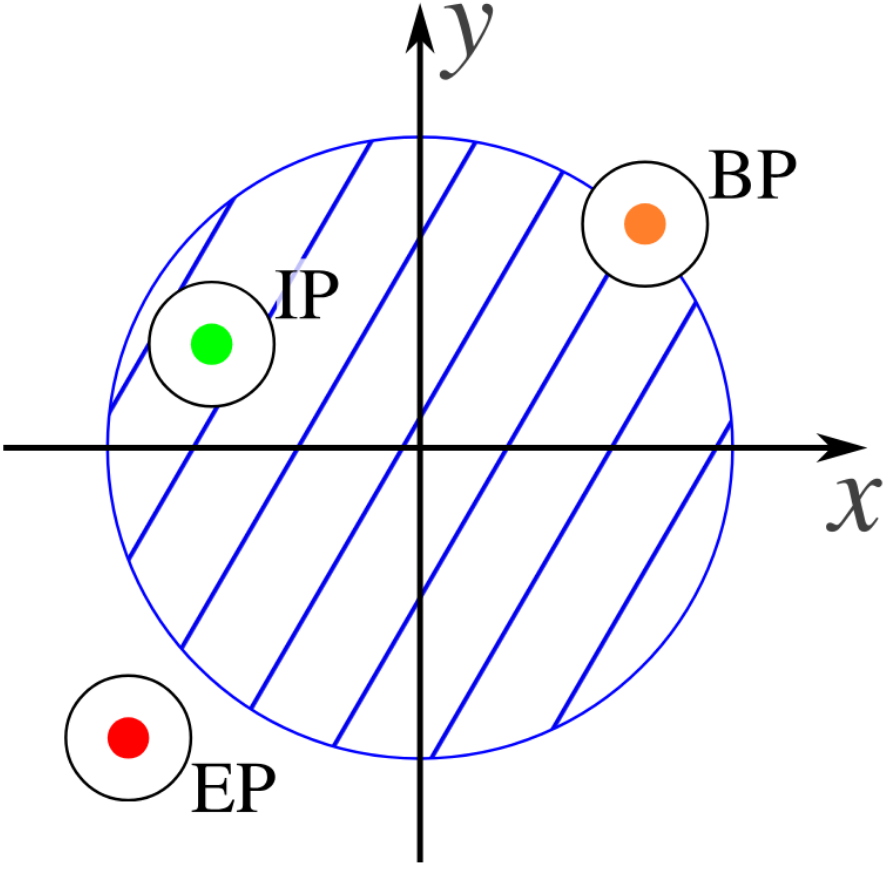
\includegraphics[width=0.5\textwidth]{ball.png}
	\caption{Interior point (IP), exterior point (EP), and boundary point (BP).}
	\label{fig:ball}
\end{figure}
Now that we have defined completeness, let us look at the difference between open and closed sets, particularly on the 2D plane. We will be considering a ball in the 2D plane,
defined,
\begin{Definitions}{Ball}{}
	A ball of radius $\epsilon$ around a point $\vb{r}_0$ is the set of all points $\vb{r}$ such that $\norm{\vb{r} - \vb{r}_0}$.
\end{Definitions} 
A sphere is the points where $\norm{\vb{r} - \vb{r}_0} = \epsilon$. Let us denote the set of the sphere $S$. We will consider three types of points, visualised in figure \ref{fig:ball},
\begin{itemize}
	\item \textbf{Exterior point}, for some $\epsilon$, all  $\vb{r} \notin S$.
	\item \textbf{Interior point}, for some $\epsilon$, all $\vb{r} \in S$.
	\item \textbf{Boundary point}, for some $\epsilon$, some of the neighbourhood of $\vb{r} \in S$ and some $\vb{r} \notin S$.
\end{itemize}
We can then define closed and open sets.
\begin{Definitions}{Closed Set}{}
	A set that contains all its boundary points is closed.
\end{Definitions}
An example of this is a set of points $\abs{r} \leq 1$, as $|r| = 1$ is a boundary point, and also belongs to the set. 
\begin{Definitions}{Open Set}{}
	A set that only includes interior points is open.
\end{Definitions}
We must furthmore define,
\begin{Definitions}{Connected Set}{}
	Sets for which any two points can be joined by a continuous path. 
\end{Definitions}
If a set is connected and open, we call it a \textit{region}.
\begin{Examples}{}
	The function $f(z) = \frac{1}{(1-z)}$ has a defined Taylor series for $z \neq 1$,
	\begin{equation}
		f(z) = \sum_{i=0}^{\infty}z^i.
	\end{equation}
	For what complex numbers is this series Cauchy? Is this an open or closed set?
\end{Examples}
We will consider the cases $|z| < 1$ and $|z| > 1$ separately, with $|z| =1$ as a boundary case. Let us define,
\begin{equation}
	a_n = \sum_{i=0}^n z^i.
\end{equation}
For any $z \neq 1$, assuming $n > m$,
\begin{equation}
	\abs{a_n - a_m} = \abs{\sum_{i = m+1}^n z_i } = \abs{\frac{z^{m+1}-z^{n+1}}{1-z}}.
\end{equation}
For $|z| < 1$,
\begin{equation}
	|a_n - a_m| = \frac{|z|^m}{|1-z|}\abs{1 - z^{n-m+1}}\leq \frac{2}{|1-z|}|z|^m
\end{equation}
and since $|z|^m$ is decreasing as a function of $m$, the series is Cauchy. For $|z|>1$,
\begin{equation}
	|a_n - a_m| = \frac{|z|^n}{|1-z|}\abs{1 - z^{-n+m+1}}\geq \frac{2}{|1-\frac{1}{z}|}|z|^n = z^{n+1}
\end{equation}
and since $|z|^{n}$ is an increasing function of $n$, the series is not Cauchy. Thus the series is Cauchy in the open set $|z| < 1$.
\chapter{Inner Product Space}
An inner product space is a vector space with an inner product, which is a generalisation of the scalar product.
\begin{Definitions}{Inner product, $\innerproduct{\vb{a}}{\vb{b}}$}{}
	Given a vector space $V_N$ over $\mathbb{F}$, the inner product between two vectors $\vb{a},\vb{b} \in V_N$ is a function such that $V \times V \to \mathbb{F}$. If $\mathbb{F} \subset \mathbb{C}$, the following properties hold,
	\begin{enumerate}
		\item \textbf{Linearity}. If $\vb{w} = \lambda\vb{u} + \mu\vb{v}$ then $\innerproduct{\vb{a}}{\vb{w}} = \lambda\innerproduct{\vb{a}}{\vb{u}} + \mu \innerproduct{\vb{a}}{\vb{u}}$.
		\item \textbf{Conjugation Symmetry.} $\overline{\innerproduct{\vb{w}}{\vb{a}}} = \innerproduct{\vb{a}}{\vb{w}}$
		\item \textbf{Positive Definiteness.} $\forall \vb{x}\neq0, \innerproduct{\vb{x}}{\vb{x}} > 0$.
	\end{enumerate}
\end{Definitions}
From our definition of the inner product, we can define the 2-norm,
\begin{equation}
	\norm{\vb{a}}^2 = \innerproduct{\vb{a}}{\vb{a}} \geq 0.
\end{equation}
\section{Orthogonality}
\begin{Definitions}{Orthogonality}{}
	$\forall \vb{a},\vb{b} \neq 0 \in V_N$ if $\innerproduct{\vb{a}}{\vb{b}} = 0$ then $\vb{a}$ and $\vb{b}$ are orthogonal.
\end{Definitions}
This allows us to then define an orthonormal basis.
\begin{Definitions}{Orthonormal basis}{}
	The set basis vectors $\left\{\vb{e}_i\right\}_{i=1}^N \in V_N$ is orthogonal if,
	\begin{equation}
		\innerproduct{\vb{e}_i}{\vb{e}_j} = A_i\delta_{ij}.
	\end{equation}
	and $A_i \neq 0$. The set of basis vectors is orthonormal for $A_i = 1, \forall i \in \left[1,N\right]$.
\end{Definitions}
Given we can decompose any vector $\vb{a} \in V_N$ if given a complete set of basis vectors, we can define a general inner product for $V_N$ over $\mathbb{F} \subset \mathbb{C}$. Let us begin by writing the decomposition of two vectors $\vb{a},\vb{b}\in V_N$ into a set of basis vectors $\left\{\vb{e}_j\right\}_{j=1}^N$,
\begin{align}
	\vb{a} = \sum_{j=1}^Na_j\vb{e}_j && \vb{b} = \sum_{j=1}^Nb_j\vb{e}_j.
\end{align}
Then, using linearity,
\begin{equation}
	\begin{split}
		\innerproduct{\vb{a}}{\vb{b}} & = \sum_{j,k=1}^N\overline{a}_j \innerproduct{\vb{e}_j}{\vb{e}_k}b_k \\
		& = \sum_{i,j=1}^N\overline{a}_j\delta_{jk}b_k \\
		& = \sum_{j=1}^N\overline{a}_jb_j.
	\end{split}
\end{equation}
NOTE: This only holds when using an orthonormal basis.
\\\\
We can obtain further insight into the decomposition of a vector by considering the inner product,
\begin{equation}
	\begin{split}
		\vb{a} = \sum_{j=1}^Na_j\vb{e}_j \implies \innerproduct{\vb{e}_k}{\vb{a}} & = \sum_{j=1}^Na_j\underbrace{\innerproduct{\vb{e}_j}{\vb{e}_k}}_{\delta_{jk}} = a_k.
	\end{split}
\end{equation}
We often refer to $a_k = \innerproduct{\vb{e}_k}{\vb{a}}$ as the \textit{projection} of $\vb{a}$ onto $\vb{e}_k$ as it gives the component of $\vb{a}$ in the $\vb{e}_k$ direction.
\section{Gram-Schmidt Orthonormalisation}
\begin{Definitions}{Gram-Schmidt Algorithm}{}
	Given a basis $\left\{\vb{v}_j\right\}_{j=1}^N \in V_N$,
	\begin{itemize}
		\item[1.] Define
		\begin{equation}
			\vb{e}_1 = \frac{\vb{v}_1}{\norm{\vb{v}_1}}
		\end{equation}
		\item[2.] Define 
		\begin{align}
			\vb{u}_2 = \vb{v}_2 - \innerproduct{\vb{e}_1}{\vb{e}_2}\vb{e_1}
	&&
			\vb{e}_2 = \frac{\vb{u}_2}{\norm{\vb{u}_2}}
		\end{align}
		\item[\vdots]
		\item[m.] Define,
		\begin{equation}
			\vb{u}_m = \vb{v}_m - \sum_{j=1}^{m-1}\innerproduct{\vb{e}_j}{\vb{v}_m}\vb{e}_j
		\end{equation}
		thus,
		\begin{equation}
			\vb{e}_m = \frac{\vb{u}_m}{\norm{\vb{u}_m}}
		\end{equation}
	\end{itemize}
	up to $N$.
\end{Definitions}
The Gram-Schmidt process is able to take any set of basis vectors and turn it into a set of orthonormal basis vectors. The idea behind it is that given 2 vectors $\vb{v},\vb{u}$ such that $\norm{\vb{u}} = 1$, then we wish to define a vector $\vb{v}' = \vb{v} - \innerproduct{\vb{u}}{\vb{v}}\vb{u}$. The inner product with $\vb{u}$ and this new vector is then,
\begin{equation}
	\innerproduct{\vb{u}}{\vb{v}'} = \innerproduct{\vb{u}}{\vb{v}} - \innerproduct{\vb{u}}{\vb{v}}\cancelto{1}{\innerproduct{\vb{u}}{\vb{u}}} = 0.
\end{equation}
So, we essentially are removing the non-orthonormal components from each subsequent basis vector, based on the first basis vector in the set.
\section{Inequalities of Inner Product Space}
\begin{Theorems}{Cauchy-Schwartz Inequality}{}
	$\forall \vb{a},\vb{b} \in V_N, \abs{\innerproduct{\vb{a}}{\vb{b}}} \leq \norm{\vb{a}}\norm{\vb{b}}$.
\end{Theorems}
\begin{proof}
	Consider $\vb{u} = \vb{a} - \lambda\vb{b}$,
	\begin{equation}
		\norm{\vb{a}}^2 = \norm{\vb{a}}^2 + |\lambda|^2\norm{\vb{b}}^2 - \overline{\lambda}\innerproduct{\vb{b}}{\vb{a}} - \lambda\innerproduct{\vb{a}}{\vb{b}} \geq 0.
	\end{equation}
Choose, 
\begin{equation}
	\lambda = \frac{\innerproduct{\vb{b}}{\vb{a}}}{\norm{\vb{b}}^2}.
\end{equation}
Thus,
\begin{equation}
	\begin{split}
		\norm{\vb{u}}^2 = \norm{\vb{a}}^2 \norm{\vb{b}}^2 - \frac{\abs{\innerproduct{\vb{a}}{\vb{b}}}}{\norm{\vb{b}}^2} \geq 0
	\end{split}
\end{equation}
$\implies \abs{\innerproduct{\vb{a}}{\vb{b}}} \leq \norm{\vb{a}}\norm{\vb{b}}$.
\end{proof}
\begin{Theorems}{Triangle Inequality}{}
	$\forall \vb{a},\vb{b} \in V_N, \norm{\vb{a} + \vb{b}}  \leq \norm{\vb{a}}\norm{\vb{b}}$
\end{Theorems}
\begin{proof}
	
\end{proof}

\end{document}
